% ============================================================
%  يُترجَم بـ XeLaTeX  (في Overleaf: Menu → Compiler → XeLaTeX)
%  الخط: Amiri (متوفر في Overleaf، أو حمّله من github.com/aliftype/amiri)
% ============================================================
\documentclass[12pt,a4paper]{article}
\usepackage[a4paper,margin=1.7cm,top=2.3cm,bottom=2.9cm,headheight=15pt,footskip=1.5cm]{geometry}
\usepackage{amsmath,amssymb}
\usepackage{icomma}
\usepackage[english,bidi=default,layout=lists]{babel}
\babelprovide[import,main]{arabic}
\babelfont{rm}[Scale=1.08]{Amiri}
\babelfont{sf}[Scale=1.08]{Amiri}
\usepackage[most]{tcolorbox}
\usepackage{tikz}
\usetikzlibrary{arrows.meta,calc,shadings}
\usepackage{array}
\usepackage{colortbl}
\usepackage{fancyhdr}
\usepackage{titlesec}
\usepackage{enumitem}
\usepackage{collcell}
\usepackage{needspace}
\usepackage{etoolbox}
\newcolumntype{C}{>{\collectcell\ar}c<{\endcollectcell}}
\pretocmd{\section}{\Needspace{15\baselineskip}}{}{}
\pretocmd{\subsection}{\Needspace{11\baselineskip}}{}{}

\definecolor{cDef}{HTML}{1F4E9C}
\definecolor{cThm}{HTML}{B3261E}
\definecolor{cRem}{HTML}{2E7D32}
\definecolor{cEx}{HTML}{C76B00}
\definecolor{cMeth}{HTML}{6A1B9A}
\definecolor{cSol}{HTML}{00695C}
\definecolor{cSec}{HTML}{1F3A68}

\titleformat{\section}{\Large\bfseries\color{cSec}}{\thesection.}{0.6em}{}[{\color{cSec!60}\titlerule[1pt]}]
\titleformat{\subsection}{\large\bfseries\color{cThm!85!black}}{\thesubsection.}{0.5em}{}
\titlespacing*{\section}{0pt}{14pt}{8pt}
\titlespacing*{\subsection}{0pt}{10pt}{5pt}
\setlength{\parindent}{0pt}
\setlength{\parskip}{4pt}
\setlist{itemsep=2pt,topsep=3pt}

\newtcolorbox{arbox}[3][]{enhanced,
  colback=#2!5,colframe=#2!80!black,arc=2mm,boxrule=0.8pt,
  left=6pt,right=6pt,top=8pt,bottom=5pt,
  fonttitle=\bfseries,coltitle=white,
  title={\foreignlanguage{arabic}{#3}},
  attach boxed title to top right={xshift=-5mm,yshift=-3mm},
  boxed title style={colback=#2!80!black,arc=1.5mm,boxrule=0pt},
  before upper={\selectlanguage{arabic}},
  before skip=8pt,after skip=8pt,breakable,#1}
\newenvironment{BOX}[2]{\begin{otherlanguage}{english}\begin{arbox}{#1}{#2}}{\end{arbox}\end{otherlanguage}}
\newenvironment{tarif}[1][تعريف]{\begin{BOX}{cDef}{#1}}{\end{BOX}}
\newenvironment{khassia}[1][خاصية]{\begin{BOX}{cThm}{#1}}{\end{BOX}}
\newenvironment{molahada}[1][ملاحظة]{\begin{BOX}{cRem}{#1}}{\end{BOX}}
\newenvironment{mithal}[1][مثال]{\begin{BOX}{cEx}{#1}}{\end{BOX}}
\newenvironment{tariqa}[1][طريقة]{\begin{BOX}{cMeth}{#1}}{\end{BOX}}

\newcounter{exo}
\newenvironment{tamrin}[1]{\stepcounter{exo}\begin{BOX}{cSec}{التمرين \theexo: #1}}{\end{BOX}}
\newenvironment{hal}{\Needspace{12\baselineskip}\begin{otherlanguage}{english}\begin{arbox}[breakable]{cSol}{حل التمرين \theexo}}{\end{arbox}\end{otherlanguage}}

\newenvironment{LTR}{\begin{otherlanguage}{english}}{\end{otherlanguage}}
\newcommand{\ar}[1]{\foreignlanguage{arabic}{#1}}

\renewcommand{\dots}{\mathinner{\ldotp\ldotp\ldotp}}
\renewcommand{\ldots}{\mathinner{\ldotp\ldotp\ldotp}}
\renewcommand{\cdots}{\mathinner{\cdotp\cdotp\cdotp}}
\newcommand{\N}{\mathbb{N}}
\newcommand{\Z}{\mathbb{Z}}
\newcommand{\D}{\mathbb{D}}
\newcommand{\Q}{\mathbb{Q}}
\newcommand{\R}{\mathbb{R}}
\newcommand{\pgcd}{\operatorname{PGCD}}
\newcommand{\ppcm}{\operatorname{PPCM}}

% \NLseg{a}{b}{[}{]} ; \NLright{a}{[} ; \NLleft{b}{]}  (interval on a number line)
\newcommand{\NLseg}[4]{\begin{LTR}\begin{tikzpicture}[baseline=-0.6ex]
 \draw[-{Stealth[length=2mm]},gray!70](0,0)--(3.4,0);
 \draw[line width=2pt,cThm!80!black](0.7,0)--(2.7,0);
 \node[cThm!80!black,font=\LARGE] at (0.7,0){$#3$};
 \node[cThm!80!black,font=\LARGE] at (2.7,0){$#4$};
 \node[below=3pt,font=\footnotesize] at (0.7,0){$#1$};
 \node[below=3pt,font=\footnotesize] at (2.7,0){$#2$};
\end{tikzpicture}\end{LTR}}
\newcommand{\NLright}[2]{\begin{LTR}\begin{tikzpicture}[baseline=-0.6ex]
 \draw[-{Stealth[length=2mm]},gray!70](0,0)--(3.4,0);
 \draw[line width=2pt,cThm!80!black](1.3,0)--(3.3,0);
 \node[cThm!80!black,font=\LARGE] at (1.3,0){$#2$};
 \node[below=3pt,font=\footnotesize] at (1.3,0){$#1$};
\end{tikzpicture}\end{LTR}}
\newcommand{\NLleft}[2]{\begin{LTR}\begin{tikzpicture}[baseline=-0.6ex]
 \draw[-{Stealth[length=2mm]},gray!70](0,0)--(3.4,0);
 \draw[line width=2pt,cThm!80!black](0.05,0)--(2.1,0);
 \node[cThm!80!black,font=\LARGE] at (2.1,0){$#2$};
 \node[below=3pt,font=\footnotesize] at (2.1,0){$#1$};
\end{tikzpicture}\end{LTR}}

% ---------- social-media icons (pure TikZ) ----------
\definecolor{cFB}{HTML}{1877F2}
\definecolor{cTG}{HTML}{229ED9}
\definecolor{cIG1}{HTML}{FEDA75}
\definecolor{cIG2}{HTML}{D62976}
\definecolor{cIG3}{HTML}{4F5BD5}
\newcommand{\fbicon}{\begin{LTR}\begin{tikzpicture}[baseline=-0.75ex,x=1em,y=1em]
 \fill[cFB] (0,0) circle (0.55);
 \node[white,inner sep=0,font=\usefont{TU}{lmss}{bx}{n}\small] at (0.04,-0.02) {f};
\end{tikzpicture}\end{LTR}}
\newcommand{\igicon}{\begin{LTR}
\begin{tikzpicture}[baseline=-0.75ex,x=1em,y=1em]
 \shade[lower left=cIG1,lower right=cIG2,upper left=cIG2,upper right=cIG3,rounded corners=0.28em] (-0.55,-0.55) rectangle (0.55,0.55);
 \draw[white,line width=0.09em,rounded corners=0.18em] (-0.36,-0.36) rectangle (0.36,0.36);
 \draw[white,line width=0.09em] (0,0) circle (0.17);
 \fill[white] (0.22,0.22) circle (0.05);
\end{tikzpicture}\end{LTR}}
\newcommand{\tgicon}{\begin{LTR}
\begin{tikzpicture}[baseline=-0.75ex,x=1em,y=1em]
 \fill[cTG] (0,0) circle (0.55);
 \fill[white] (-0.33,0.0) -- (0.32,0.27) -- (0.2,-0.3) -- (0.0,-0.15) -- (-0.08,-0.28) -- (-0.08,-0.08) -- cycle;
 \fill[cTG!70!black] (-0.08,-0.08) -- (0.25,0.2) -- (0.0,-0.15) -- (-0.08,-0.28) -- cycle;
\end{tikzpicture}\end{LTR}}
% page number: black box, white two-digit number, at the right of the social row
\newcommand{\PageBox}{\begin{LTR}\tikz[baseline=(p.base)]\node[fill=black,text=white,inner sep=2.5pt,minimum width=1.6em,minimum height=1.3em,font=\usefont{TU}{lmss}{bx}{n}\small](p){\ifnum\value{page}<10 0\fi\arabic{page}};\end{LTR}}
% visual left-to-right order: Telegram | Instagram | Facebook | page box
\newcommand{\SocialRow}{\begin{otherlanguage}{english}%
 \ar{\textbf{الأستاذ سوايسية هشام للرياضيات}}\ \tgicon\hfill
 \textbf{prof\_hicham\_math}\ \igicon\hfill
 \ar{\textbf{الأستاذ سوايسية هشام للرياضيات}}\ \fbicon\hspace{2.2em}\PageBox\end{otherlanguage}}

\pagestyle{fancy}
\fancyhf{}
\renewcommand{\headrulewidth}{0.6pt}
\renewcommand{\footrulewidth}{0.4pt}
% \SetHeader{right head: document title}{left head: level -- stream}
\newcommand{\SetHeader}[2]{%
 \fancyhead[C]{\parbox{\textwidth}{\ar{#1\hfill #2}}}%
 \fancyfoot[C]{\parbox{\textwidth}{\small\SocialRow}}}
\usepackage{tkz-tab}
\usepackage{multicol}
% variation / sign table (LTR)
\newenvironment{TAB}{\par\begin{center}\begin{LTR}\begin{tikzpicture}[scale=0.95,every node/.style={font=\small}]}{\end{tikzpicture}\end{LTR}\end{center}}
% grid + axes, clipped: \begin{GR}{xmin}{xmax}{ymin}{ymax}{unit cm}
\newenvironment{GR}[5]{\par\begin{center}\begin{LTR}\begin{tikzpicture}[x=#5cm,y=#5cm,font=\footnotesize]
 \draw[gray!25,very thin] (#1,#3) grid (#2,#4);
 \draw[-{Stealth[length=2mm]}] (#1,0)--(#2+0.3,0) node[below left]{$x$};
 \draw[-{Stealth[length=2mm]}] (0,#3)--(0,#4+0.3) node[below left]{$y$};
 \node[below left] at (0,0){$O$};
 \begin{scope}\clip (#1,#3) rectangle (#2,#4);}
{\end{scope}\end{tikzpicture}\end{LTR}\end{center}}
\newcommand{\Ticks}[2]{\foreach \t in {#1} \node[below,font=\scriptsize] at (\t,0){$\t$}; \foreach \t in {#2} \node[left,font=\scriptsize] at (0,\t){$\t$};}
\newcommand{\bx}[1]{\ensuremath{\colorbox{cDef!12}{$\displaystyle #1$}}}
\newcommand{\TwoCol}[4]{\par\begin{LTR}\noindent\begin{minipage}[t]{#1\textwidth}\selectlanguage{arabic}#2\end{minipage}\hfill\begin{minipage}[t]{#3\textwidth}\selectlanguage{arabic}#4\end{minipage}\end{LTR}\par}
\newcommand{\RL}[4]{\TwoCol{#3}{#4}{#1}{#2}}  % \RL{w1}{right content}{w2}{left content}
\newcommand{\ok}{$\textcolor{cRem}{\checkmark}$}
\newcommand{\limn}{\displaystyle\lim_{n\to+\infty}}
% sub-questions, each on its own line
\newenvironment{sq}{\begin{itemize}[leftmargin=2.4em,itemsep=3pt]}{\end{itemize}}
\newcommand{\qa}{\item[(أ)]}\newcommand{\qb}{\item[(ب)]}\newcommand{\qc}{\item[(جـ)]}\newcommand{\qd}{\item[(د)]}\newcommand{\qe}{\item[(هـ)]}
\newcommand{\pa}{\par\smallskip\textbf{(أ)} }\newcommand{\pb}{\par\smallskip\textbf{(ب)} }\newcommand{\pc}{\par\smallskip\textbf{(جـ)} }\newcommand{\pd}{\par\smallskip\textbf{(د)} }\newcommand{\pe}{\par\smallskip\textbf{(هـ)} }
\newcommand{\QQ}[1]{\par\smallskip\textbf{#1.} }
\newenvironment{tmr}{\stepcounter{exo}\begin{BOX}{cSec}{تمرين محلول \theexo}}{\end{BOX}}
\newcommand{\ABC}[3]{\\[2pt]\begin{tabular}{p{0.28\textwidth}p{0.28\textwidth}p{0.28\textwidth}}(جـ) \ #3 & (ب) \ #2 & (أ) \ #1\end{tabular}}
\pretocmd{\section}{\Needspace{24\baselineskip}}{}{}
\newtcbox{\bxtbox}{on line,colback=cDef!12,colframe=cDef!12,boxrule=0pt,arc=1pt,boxsep=0pt,left=2pt,right=2pt,top=1pt,bottom=1pt}
\newcommand{\bxt}[1]{\foreignlanguage{english}{\bxtbox{\ar{#1}}}}
\SetHeader{\small\bfseries\color{cSec}ملخص: الدوال الأصلية والحساب التكاملي}{\small\color{cSec}السنة الثالثة ثانوي -- تسيير واقتصاد}
\let\origNeedspace\Needspace
\renewcommand{\Needspace}[1]{\origNeedspace{14\baselineskip}}
% graph paper: \Paper{width}{height} (dimensions with units), origin at (0,0)
\newcommand{\Paper}[2]{%
 \fill[orange!4] (0cm,0cm) rectangle (#1,#2);
 \draw[orange!22,very thin,step=1mm] (0cm,0cm) grid (#1,#2);
 \draw[orange!40,thin,step=5mm] (0cm,0cm) grid (#1,#2);
 \draw[orange!65,step=1cm] (0cm,0cm) grid (#1,#2);}
\newcommand{\Pt}[1]{\fill[cThm] #1 circle (2.2pt);}
\newenvironment{FIG}{\par\begin{center}\begin{LTR}}{\end{LTR}\end{center}}
\renewcommand{\arraystretch}{1.25}
\begin{document}
\begin{LTR}
\begin{tcolorbox}[enhanced,colback=cSec,colframe=cSec,arc=3mm,halign=center,boxrule=0pt,top=12pt,bottom=12pt,before upper={\selectlanguage{arabic}}]
{\color{white}\fontsize{26}{32}\selectfont\bfseries الدوال الأصلية والحساب التكاملي}\\[8pt]
{\color{white}\large ملخص شامل مع أمثلة وأشكال وتمارين محلولة خطوة بخطوة}\\[5pt]
{\color{white}\large السنة الثالثة ثانوي -- تسيير واقتصاد}
\end{tcolorbox}
\end{LTR}

\begin{BOX}{cSec}{محتوى الملخص}
\begin{enumerate}[label=\textbf{\arabic*.}]
\item الدالة الأصلية لدالة على مجال، والدوال الأصلية لدوال مألوفة.
\item الدوال الأصلية والعمليات على الدوال.
\item دالة أصلية تحقق شرطًا معيّنًا، والتطبيق الاقتصادي (الكلفة الهامشية والكلفة الإجمالية).
\item تكامل دالة: من المساحة إلى الكتابة $\int_a^bf(t)\,dt$.
\item خواص التكامل: الخطية، علاقة شال، الترتيب.
\item القيمة المتوسطة لدالة على مجال وتفسيرها.
\item حساب المساحات: منحنٍ ومحور الفواصل، ثم بين منحنيين.
\item تمرينان محلولان، أخطاء شائعة، ثم خلاصة الطرائق.
\end{enumerate}
\end{BOX}
%================================================================
\section{الدالة الأصلية لدالة على مجال}
\begin{tarif}
$f$ دالة معرفة على مجال $I$. نسمي \textbf{دالة أصلية} للدالة $f$ على $I$ كل دالة $F$ قابلة للاشتقاق على $I$ وتحقق:
\begin{center}\bx{F'(x)=f(x)} \ من أجل كل $x$ من $I$\end{center}
البحث عن دالة أصلية هو «عكس» عملية الاشتقاق.
\end{tarif}

\begin{mithal}
الدوال $x^2$ ، $x^2+1$ ، $x^2-7$ كلها مشتقتها $2x$: هي دوال أصلية للدالة $x\mapsto2x$ على $\mathbb R$، والفرق بين اثنتين منها \textbf{عدد ثابت}.
\end{mithal}

\begin{khassia}
\begin{enumerate}[label=\textbf{\arabic*.}]
\item كل دالة \textbf{مستمرة} على مجال $I$ تقبل دوالًا أصلية على $I$.
\item إذا كانت $F$ دالة أصلية لـ $f$ على $I$ فإن كل الدوال الأصلية لـ $f$ على $I$ هي الدوال \bx{x\mapsto F(x)+c} حيث $c$ عدد حقيقي ثابت.
\item إذا كانت $F$ و$G$ دالتين أصليتين لـ $f$ و$g$ على $I$ فإن $F+G$ دالة أصلية لـ $f+g$، و$kF$ دالة أصلية لـ $kf$ حيث $k$ عدد حقيقي.
\end{enumerate}
\end{khassia}

\begin{tariqa}[التحقق أن $F$ دالة أصلية لـ $f$]
نحسب $F'(x)$ ونبيّن أن $F'(x)=f(x)$ من أجل كل $x$ من $I$.
\end{tariqa}

\begin{mithal}
بيّن أن $F(x)=x^3-2x^2+5$ دالة أصلية لـ $f(x)=3x^2-4x$ على $\mathbb R$:\quad
$F'(x)=3x^2-4x+0=f(x)$ \ok.
\end{mithal}

\section{الدوال الأصلية لدوال مألوفة}
\begin{khassia}[جدول الدوال الأصلية ($c$ عدد حقيقي كيفي)]
\begin{center}
\renewcommand{\arraystretch}{2}
\begin{tabular}{|C|C|C|}\hline
\rowcolor{cSec!12} المجال $I$ & الدوال الأصلية $F(x)$ & الدالة $f(x)$\\\hline
$\mathbb R$ & $ax+c$ & $a$ \ ($a$ عدد حقيقي)\\\hline
$\mathbb R$ & $\dfrac12x^2+c$ & $x$\\\hline
$\mathbb R$ & $\dfrac{1}{n+1}x^{n+1}+c$ & $x^n\ \ (n\in\mathbb N^*)$\\\hline
$]-\infty;0[$ أو $]0;+\infty[$ & $-\dfrac1x+c$ & $\dfrac1{x^2}$\\\hline
$]-\infty;0[$ أو $]0;+\infty[$ & $-\dfrac{1}{(n-1)x^{n-1}}+c$ & $\dfrac1{x^n}$ \ ($n\in\mathbb N$ و$n\ge2$)\\\hline
$]0;+\infty[$ & $2\sqrt x+c$ & $\dfrac1{\sqrt x}$\\\hline
\end{tabular}
\end{center}
\end{khassia}

\begin{mithal}[أمثلة]
\begin{enumerate}[label=\textbf{\arabic*.}]
\item $f(x)=4x^3-6x+5$ على $\mathbb R$: نطبق القاعدة على كل حد:
\[F(x)=4\times\frac{x^4}{4}-6\times\frac{x^2}{2}+5x=\bx{x^4-3x^2+5x}\]
\item $g(x)=\dfrac{3}{x^3}=3\times\dfrac1{x^3}$ على $]0;+\infty[$ ($n=3$): \ $G(x)=3\times\left(-\dfrac{1}{2x^2}\right)=\bx{-\dfrac{3}{2x^2}}$.
\item $h(x)=x^2-\dfrac2{x^2}$ على $]0;+\infty[$: \ $H(x)=\dfrac{x^3}{3}-2\times\left(-\dfrac1x\right)=\bx{\dfrac{x^3}{3}+\dfrac2x}$.
\end{enumerate}
\end{mithal}

\section{الدوال الأصلية والعمليات على الدوال}
\begin{khassia}[$u$ دالة قابلة للاشتقاق على مجال $I$]
\begin{center}
\renewcommand{\arraystretch}{2.1}
\begin{tabular}{|C|C|C|}\hline
\rowcolor{cSec!12} شروط على $u$ & الدوال الأصلية & الدالة $f$\\\hline
-- & $\dfrac12u^2+c$ & $u'u$\\\hline
-- & $\dfrac{1}{n+1}u^{n+1}+c$ & $u'u^n\ \ (n\in\mathbb N^*)$\\\hline
$u(x)\neq0$ على $I$ & $-\dfrac1u+c$ & $\dfrac{u'}{u^2}$\\\hline
$u(x)\neq0$ على $I$ & $-\dfrac{1}{(n-1)u^{n-1}}+c$ & $\dfrac{u'}{u^n}\ \ (n\ge2)$\\\hline
$u(x)>0$ على $I$ & $2\sqrt u+c$ & $\dfrac{u'}{\sqrt u}$\\\hline
\end{tabular}
\end{center}
\end{khassia}

\begin{tariqa}[التعرف على الشكل]
\begin{enumerate}[label=\textbf{\arabic*.}]
\item نختار $u(x)$ (ما داخل القوس أو المقام أو الجذر) ونحسب $u'(x)$.
\item نكتب $f$ على أحد الأشكال $u'u^n$ ، $\dfrac{u'}{u^n}$ ، $\dfrac{u'}{\sqrt u}$، مع ضرب وقسمة على عدد ثابت إذا لزم.
\item نطبق القاعدة ثم نتحقق بالاشتقاق.
\end{enumerate}
\end{tariqa}

\begin{mithal}[أمثلة محلولة]
\begin{enumerate}[label=\textbf{\arabic*.}]
\item $f(x)=6x(x^2+1)^2$: \ $u(x)=x^2+1$ ، $u'(x)=2x$ ، إذن $f=3\,u'u^2$ ومنه
\[F(x)=3\times\frac{u^3}{3}=\bx{(x^2+1)^3}\]
\item $g(x)=(2x+1)(x^2+x)^2$: \ $u(x)=x^2+x$ ، $u'(x)=2x+1$ ، $g=u'u^2$ ومنه $G(x)=\bx{\dfrac{(x^2+x)^3}{3}}$.
\item $h(x)=\dfrac{3}{(3x-1)^2}$ على $\left]\frac13;+\infty\right[$: \ $u(x)=3x-1$ ، $u'(x)=3$ ، $h=\dfrac{u'}{u^2}$ ومنه $H(x)=\bx{-\dfrac{1}{3x-1}}$.
\item $k(x)=\dfrac{2x}{(x^2+1)^2}$ على $\mathbb R$: \ $u(x)=x^2+1\neq0$ ، $u'(x)=2x$ ، ومنه $K(x)=\bx{-\dfrac{1}{x^2+1}}$.
\item $m(x)=\dfrac{x}{\sqrt{x^2+4}}$ على $\mathbb R$: \ $u(x)=x^2+4>0$ ، $u'(x)=2x$ ، $m=\dfrac12\times\dfrac{u'}{\sqrt u}$ ومنه
\[M(x)=\frac12\times2\sqrt{u}=\bx{\sqrt{x^2+4}}\]
\end{enumerate}
\textbf{تحقق} (المثال 4): $K'(x)=-\dfrac{-2x}{(x^2+1)^2}=\dfrac{2x}{(x^2+1)^2}=k(x)$ \ok.
\end{mithal}

\section{دالة أصلية تحقق شرطًا معيّنًا}
\begin{khassia}
$f$ دالة تقبل دوالًا أصلية على $I$. من أجل كل عدد $x_0$ من $I$ وكل عدد حقيقي $y_0$ توجد \textbf{دالة أصلية وحيدة} $F$ لـ $f$ على $I$ تحقق \bx{F(x_0)=y_0}.
\end{khassia}

\begin{tariqa}
نكتب الدوال الأصلية $F(x)=G(x)+c$ ، نعوض الشرط $F(x_0)=y_0$ فنجد $c$ ، ثم نكتب $F$.
\end{tariqa}

\begin{mithal}
$f(x)=3x^2-2x+1$. عيّن الدالة الأصلية $F$ لـ $f$ على $\mathbb R$ التي تحقق $F(1)=4$.

$F(x)=x^3-x^2+x+c$ ؛ \ $F(1)=1-1+1+c=1+c$ \ و\ $F(1)=4$ \ ومنه $c=3$:
\[\bx{F(x)=x^3-x^2+x+3}\]
\end{mithal}

\begin{BOX}{cMeth}{تطبيق اقتصادي: الكلفة الهامشية والكلفة الإجمالية}
\begin{itemize}
\item الكلفة الهامشية هي مشتقة الكلفة الإجمالية: $C_m(q)=C'(q)$ ، إذن \textbf{الكلفة الإجمالية $C$ دالة أصلية للكلفة الهامشية $C_m$}.
\item \textbf{الكلفة الثابتة} هي $C(0)$: هي الشرط الذي يعيّن الثابت $c$.
\item الربح: $B(q)=p\,q-C(q)$ حيث $p$ ثمن بيع الوحدة.
\end{itemize}
\end{BOX}

\begin{mithal}
الكلفة الهامشية لمؤسسة $C_m(q)=3q^2-12q+20$ والكلفة الثابتة $100$.

$C(q)=q^3-6q^2+20q+c$ ؛ \ $C(0)=c=100$ ، إذن \bx{C(q)=q^3-6q^2+20q+100}.

إذا كان ثمن بيع الوحدة $68$: \ $B(q)=68q-C(q)=\bx{-q^3+6q^2+48q-100}$.
\end{mithal}

\section{تكامل دالة}
\begin{mithal}[من المساحة إلى الدالة الأصلية]
$f(t)=2t+1$ على $[1;3]$: الحيز تحت المستقيم شبه منحرف قاعدتاه $f(1)=3$ و$f(3)=7$ وارتفاعه $2$:
\begin{FIG}
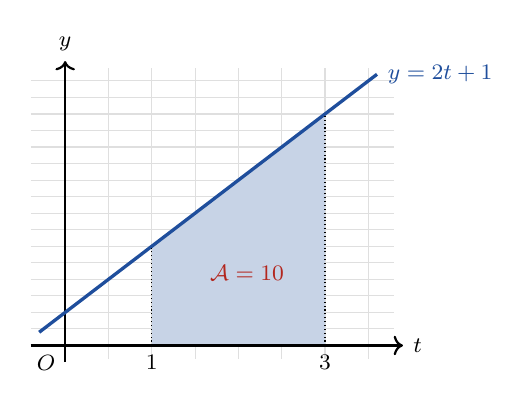
\begin{tikzpicture}[x=1.1cm,y=0.42cm,font=\footnotesize]
\draw[gray!25,step=0.5] (-0.4,-0.4) grid (3.8,8.4);
\fill[cDef!25] (1,0) -- (1,3) -- (3,7) -- (3,0) -- cycle;
\draw[->,thick] (-0.4,0)--(3.9,0) node[right]{$t$}; \draw[->,thick] (0,-0.5)--(0,8.6) node[above]{$y$};
\draw[cDef,very thick] (-0.3,0.4)--(3.6,8.2) node[right]{$y=2t+1$};
\draw[densely dotted] (1,0)--(1,3) (3,0)--(3,7);
\node[below] at (1,0){$1$}; \node[below] at (3,0){$3$}; \node[below left] at (0,0){$O$};
\node[cThm] at (2.1,2.2){$\mathcal A=10$};
\end{tikzpicture}
\end{FIG}
$\mathcal A=\dfrac{(3+7)\times2}{2}=10$. \ والدالة $F(t)=t^2+t$ دالة أصلية لـ $f$: \ $F(3)-F(1)=12-2=10$ \ \textbf{نفس النتيجة}.
\end{mithal}

\begin{tarif}
$f$ دالة مستمرة على مجال $I$، $a$ و$b$ عددان من $I$ و$F$ دالة أصلية لـ $f$ على $I$. العدد $F(b)-F(a)$ يسمى \textbf{تكامل} $f$ من $a$ إلى $b$ ونكتب:
\[\bx{\int_a^bf(t)\,dt=\Big[F(t)\Big]_a^b=F(b)-F(a)}\]
(لا يتعلق بالدالة الأصلية المختارة، لأن الثابت $c$ يختفي في الفرق.)
\end{tarif}

\begin{molahada}[دور المتغير]
المتغير $t$ «\textbf{صامت}»: يمكن تعويضه بأي حرف: $\displaystyle\int_a^bf(t)\,dt=\int_a^bf(x)\,dx=\int_a^bf(q)\,dq$. النتيجة عدد حقيقي يتعلق بـ $a$ و$b$ فقط.
\end{molahada}

\begin{khassia}[التفسير البياني]
إذا كانت $f$ \textbf{مستمرة وموجبة} على $[a;b]$ ($a\le b$) فإن $\displaystyle\int_a^bf(t)\,dt$ هو مساحة الحيز المحدد بالمنحني $(C_f)$ ومحور الفواصل والمستقيمين اللذين معادلتاهما $x=a$ و$x=b$ (بوحدة المساحات).
\end{khassia}

\begin{mithal}
\begin{minipage}{0.55\textwidth}
$\displaystyle\int_0^2t^2\,dt=\left[\frac{t^3}{3}\right]_0^2=\frac83-0=\bx{\frac83}$

هو مساحة الحيز الملوّن تحت المنحني $y=t^2$ بين $0$ و$2$.

$\displaystyle\int_1^2(3t^2-1)\,dt=\Big[t^3-t\Big]_1^2=(8-2)-(1-1)=\bx{6}$.
\end{minipage}\hfill
\begin{minipage}{0.4\textwidth}
\begin{LTR}\centering
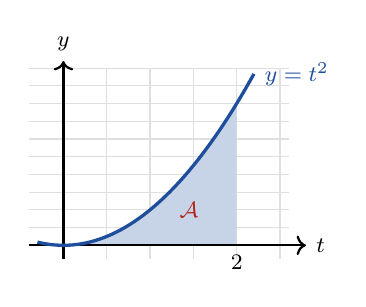
\begin{tikzpicture}[x=1.1cm,y=0.45cm,font=\footnotesize]
\draw[gray!25,step=0.5] (-0.4,-0.4) grid (2.6,5);
\fill[cDef!25] (0,0) -- plot[domain=0:2,samples=50] (\x,{\x*\x}) -- (2,0) -- cycle;
\draw[->,thick] (-0.4,0)--(2.8,0) node[right]{$t$}; \draw[->,thick] (0,-0.4)--(0,5.2) node[above]{$y$};
\draw[cDef,very thick,domain=-0.3:2.2,samples=50] plot (\x,{\x*\x}) node[right]{$y=t^2$};
\node[below] at (2,0){$2$}; \node[cThm] at (1.45,1){$\mathcal A$};
\end{tikzpicture}
\end{LTR}
\end{minipage}
\end{mithal}

\begin{mithal}[مثال اقتصادي]
الكلفة الهامشية $C_m(q)=2q+10$: \ $\displaystyle\int_0^{10}C_m(q)\,dq=\Big[q^2+10q\Big]_0^{10}=200$.

بما أن $C$ دالة أصلية لـ $C_m$: \ $\displaystyle\int_0^{10}C_m(q)\,dq=C(10)-C(0)$: هو \textbf{زيادة الكلفة الإجمالية} لما ننتقل من $0$ إلى $10$ وحدات.
\end{mithal}

\section{خواص التكامل}
\begin{khassia}[$f$ و$g$ مستمرتان على $I$ ، $a$ ، $b$ ، $c$ من $I$ ، $k$ عدد حقيقي]
\begin{enumerate}[label=\textbf{\arabic*.}]
\item $\displaystyle\int_a^af(x)\,dx=0$ \ و\ $\displaystyle\int_b^af(x)\,dx=-\int_a^bf(x)\,dx$.
\item \textbf{الخطية:}
\[\int_a^b\big[f(x)+g(x)\big]dx=\int_a^bf(x)\,dx+\int_a^bg(x)\,dx\qquad;\qquad\int_a^bk\,f(x)\,dx=k\int_a^bf(x)\,dx\]
\item \textbf{علاقة شال:} \ $\displaystyle\int_a^bf(x)\,dx+\int_b^cf(x)\,dx=\int_a^cf(x)\,dx$.
\item \textbf{الترتيب} (مع $a\le b$):
\begin{itemize}
\item إذا كان $f(x)\ge0$ على $[a;b]$ فإن $\displaystyle\int_a^bf(x)\,dx\ge0$.
\item إذا كان $f(x)\le g(x)$ على $[a;b]$ فإن $\displaystyle\int_a^bf(x)\,dx\le\int_a^bg(x)\,dx$.
\end{itemize}
\end{enumerate}
\end{khassia}

\begin{mithal}[أمثلة]
\begin{enumerate}[label=\textbf{\arabic*.}]
\item \textbf{الخطية:} $\displaystyle\int_0^1(3x^2+2x)\,dx=3\int_0^1x^2\,dx+2\int_0^1x\,dx=3\times\frac13+2\times\frac12=\bx{2}$.
\item \textbf{الترتيب:} على $[0;1]$ لدينا $x^2\le x$ ، إذن $\displaystyle\int_0^1x^2\,dx\le\int_0^1x\,dx$ ، أي $\dfrac13\le\dfrac12$ \ok.
\item \textbf{علاقة شال:} على $[0;1]$: $|x-1|=1-x$ ، وعلى $[1;3]$: $|x-1|=x-1$:
\[\int_0^3|x-1|\,dx=\int_0^1(1-x)\,dx+\int_1^3(x-1)\,dx=\frac12+2=\bx{\frac52}\]
\end{enumerate}
\end{mithal}

\section{القيمة المتوسطة لدالة على مجال}
\begin{tarif}
$f$ دالة مستمرة على $I$ ، $a$ و$b$ من $I$ حيث $a<b$. \textbf{القيمة المتوسطة} لـ $f$ على $[a;b]$ هي العدد:
\[\bx{\mu=\frac{1}{b-a}\int_a^bf(x)\,dx}\]
\end{tarif}

\begin{khassia}[التفسير البياني]
\begin{minipage}{0.55\textwidth}
إذا كانت $f$ موجبة على $[a;b]$: \ $\mu\,(b-a)=\displaystyle\int_a^bf(x)\,dx$.

أي أن \textbf{المستطيل} الذي قاعدته $b-a$ وارتفاعه $\mu$ له \textbf{نفس مساحة} الحيز تحت $(C_f)$ بين $a$ و$b$.
\end{minipage}\hfill
\begin{minipage}{0.4\textwidth}
\begin{LTR}\centering
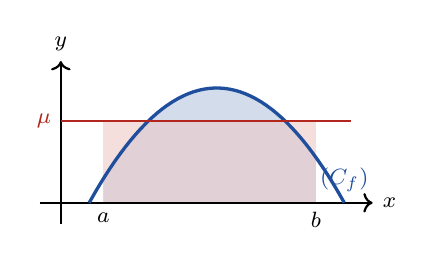
\begin{tikzpicture}[x=0.9cm,y=0.9cm,font=\footnotesize]
\fill[cDef!20] (0.6,0) -- plot[domain=0.6:3.6,samples=50] (\x,{-0.5*(\x-0.4)*(\x-4)}) -- (3.6,0) -- cycle;
\fill[cThm!25,opacity=0.6] (0.6,0) rectangle (3.6,1.15);
\draw[->,thick] (-0.3,0)--(4.4,0) node[right]{$x$}; \draw[->,thick] (0,-0.3)--(0,2.0) node[above]{$y$};
\draw[cDef,very thick,domain=0.4:4,samples=50] plot (\x,{-0.5*(\x-0.4)*(\x-4)}) node[above]{$(C_f)$};
\draw[cThm,thick] (0,1.15)--(4.1,1.15); \node[left,cThm] at (0,1.15){$\mu$};
\node[below] at (0.6,0){$a$}; \node[below] at (3.6,0){$b$};
\end{tikzpicture}
\end{LTR}
\end{minipage}
\end{khassia}

\begin{mithal}
\begin{enumerate}[label=\textbf{\arabic*.}]
\item $f(x)=3x^2-4x+1$ على $[0;2]$: \ $\displaystyle\int_0^2f(x)\,dx=\Big[x^3-2x^2+x\Big]_0^2=8-8+2=2$ ، إذن $\mu=\dfrac{1}{2-0}\times2=\bx{1}$.
\item \textbf{اقتصادي:} $C_m(q)=2q+10$ على $[10;20]$:
\[\mu=\frac{1}{20-10}\Big[q^2+10q\Big]_{10}^{20}=\frac{600-200}{10}=\bx{40}\]
هو \textbf{متوسط الكلفة الهامشية} لما يتغير الإنتاج من $10$ إلى $20$ وحدة.
\end{enumerate}
\end{mithal}

\section{حساب المساحات}
\begin{tarif}[وحدة المساحات]
في معلم متعامد $(O;\vec i,\vec j)$، وحدة المساحات $\text{u.a}$ هي مساحة المستطيل الذي بعداه $\|\vec i\|$ و$\|\vec j\|$. مثلا: إذا كان $\|\vec i\|=2\,\text{cm}$ و$\|\vec j\|=1\,\text{cm}$ فإن \bx{1\ \text{u.a}=2\,\text{cm}^2}.
\end{tarif}

\begin{khassia}[مساحة الحيز بين منحنٍ ومحور الفواصل والمستقيمين $x=a$ و$x=b$ ($a<b$)]
\begin{enumerate}[label=\textbf{\arabic*.}]
\item إذا كانت $f(x)\ge0$ على $[a;b]$ ($(C_f)$ فوق محور الفواصل): \ \bx{\mathcal A=\int_a^bf(x)\,dx}.
\item إذا كانت $f(x)\le0$ على $[a;b]$ ($(C_f)$ تحت محور الفواصل): \ \bx{\mathcal A=-\int_a^bf(x)\,dx}.
\item إذا تغيرت إشارة $f$: نقسم المجال عند النقط التي تنعدم فيها $f$ (علاقة شال) ونجمع المساحات.
\end{enumerate}
\end{khassia}

\begin{khassia}[مساحة الحيز بين منحنيين]
إذا كان $f(x)\ge g(x)$ على $[a;b]$ ($(C_f)$ فوق $(C_g)$) فإن مساحة الحيز المحدد بالمنحنيين والمستقيمين $x=a$ و$x=b$ هي:
\[\bx{\mathcal A=\int_a^b\big[f(x)-g(x)\big]\,dx}\]
\end{khassia}

\begin{tariqa}[خطوات حساب مساحة]
\begin{enumerate}[label=\textbf{\arabic*.}]
\item نعيّن نقط التقاطع (حلول $f(x)=0$ أو $f(x)=g(x)$).
\item ندرس إشارة $f(x)$ (أو $f(x)-g(x)$) في \textbf{جدول الوضع النسبي}.
\item نرسم المنحنيات ونلوّن الحيز (لون مختلف لكل جزء).
\item نحسب التكامل (الأعلى ناقص الأسفل) بوحدة المساحات $\text{u.a}$ ثم نحوّل إلى $\text{cm}^2$ إذا طُلب.
\end{enumerate}
\end{tariqa}

\begin{mithal}[مثال 1: منحنٍ يغيّر إشارته]
$f(x)=x^2-1$. \ احسب مساحة الحيز المحدد بـ $(C_f)$ ومحور الفواصل والمستقيمين $x=0$ و$x=2$.

\textbf{الوضع النسبي:} $f(x)=(x-1)(x+1)$:
\begin{FIG}
\begin{tikzpicture}[font=\normalsize]
\fill[gray!12] (0,0) rectangle (2.6,-0.9);
\fill[green!18] (2.6,0) rectangle (15.5,-0.9);
\fill[orange!45] (0,-0.9) rectangle (2.6,-4.6);
\fill[cyan!22] (2.6,-0.9) rectangle (15.5,-4.6);
\draw[thick] (0,0) rectangle (15.5,-4.6); \draw (0,-0.9)--(15.5,-0.9) (0,-1.8)--(15.5,-1.8) (2.6,0)--(2.6,-4.6);
\node at (1.3,-0.45){$x$};
\node at (1.3,-1.35){$f(x)$};
\node[align=center,font=\bfseries] at (1.3,-3.2){\ar{الوضع}\\ \ar{النسبي}};
\node at (3.3,-0.45){$0$};
\node at (9.05,-0.45){$1$};
\node at (14.8,-0.45){$2$};
\node at (5.425,-1.35){$-$};
\node[align=center,font=\small] at (5.425,-3.2){$(C_f)$\\ \ar{تحت}\\ $(xx')$};
\node at (12.675,-1.35){$+$};
\node[align=center,font=\small] at (12.675,-3.2){$(C_f)$\\ \ar{فوق}\\ $(xx')$};
\node at (9.05,-1.35){$0$};
\draw[densely dotted] (9.05,-0.9)--(9.05,-1.13) (9.05,-1.57)--(9.05,-1.8);
\draw (7.55,-4.6) .. controls (7.625,-3.06) and (8.6,-2.136) .. (9.05,-1.8) .. controls (9.5,-2.136) and (10.475,-3.06) .. (10.55,-4.6);
\node[align=center,font=\footnotesize,inner sep=0pt] at (9.05,-3.65){\ar{$(C_f)$ يقطع}\\ $(xx')$\\ \ar{في النقطة}\\ $A(1;0)$};
\end{tikzpicture}
\end{FIG}
\begin{FIG}
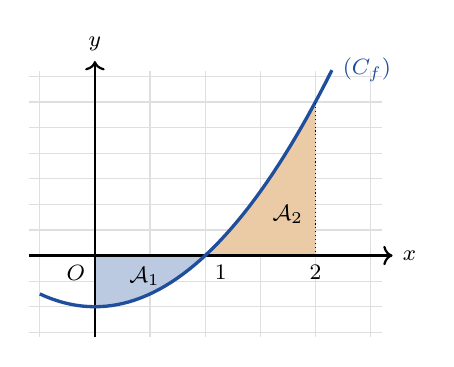
\begin{tikzpicture}[x=1.4cm,y=0.65cm,font=\footnotesize]
\draw[gray!25,step=0.5] (-0.6,-1.6) grid (2.6,3.6);
\fill[cDef!30] (0,0) -- plot[domain=0:1,samples=40] (\x,{\x*\x-1}) -- cycle;
\fill[cEx!35] (1,0) -- plot[domain=1:2,samples=40] (\x,{\x*\x-1}) -- (2,0) -- cycle;
\draw[->,thick] (-0.6,0)--(2.7,0) node[right]{$x$}; \draw[->,thick] (0,-1.6)--(0,3.8) node[above]{$y$};
\draw[cDef,very thick,domain=-0.5:2.15,samples=50] plot (\x,{\x*\x-1}) node[right]{$(C_f)$};
\draw[densely dotted] (2,0)--(2,3);
\node[below right] at (1,0){$1$}; \node[below] at (2,0){$2$}; \node[below left] at (0,0){$O$};
\node at (0.45,-0.4){$\mathcal A_1$}; \node at (1.75,0.8){$\mathcal A_2$};
\end{tikzpicture}
\end{FIG}
\[\mathcal A_1=-\int_0^1(x^2-1)\,dx=-\left[\frac{x^3}{3}-x\right]_0^1=-\left(\frac13-1\right)=\frac23\]
\[\mathcal A_2=\int_1^2(x^2-1)\,dx=\left(\frac83-2\right)-\left(\frac13-1\right)=\frac23+\frac23=\frac43\]
\[\bx{\mathcal A=\mathcal A_1+\mathcal A_2=\frac23+\frac43=2\ \text{u.a}}\]
\textbf{انتبه:} $\displaystyle\int_0^2(x^2-1)\,dx=\frac23$ ليس هو المساحة، لأن الجزء تحت محور الفواصل «يُطرح».
\end{mithal}

\begin{mithal}[مثال 2: بين منحنيين]
$f(x)=-x^2+4x$ و$g(x)=x$. \ احسب مساحة الحيز المحصور بين $(C_f)$ و$(C_g)$.

\textbf{التقاطع:} $-x^2+4x=x$ معناه $x(3-x)=0$: \ $x=0$ أو $x=3$. \quad \textbf{الوضع النسبي:} $f(x)-g(x)=x(3-x)$:
\begin{FIG}
\begin{tikzpicture}[font=\normalsize]
\fill[gray!12] (0,0) rectangle (2.6,-0.9);
\fill[green!18] (2.6,0) rectangle (15.5,-0.9);
\fill[orange!45] (0,-0.9) rectangle (2.6,-4.6);
\fill[cyan!22] (2.6,-0.9) rectangle (15.5,-4.6);
\draw[thick] (0,0) rectangle (15.5,-4.6); \draw (0,-0.9)--(15.5,-0.9) (0,-1.8)--(15.5,-1.8) (2.6,0)--(2.6,-4.6);
\node at (1.3,-0.45){$x$};
\node at (1.3,-1.35){$f(x)-g(x)$};
\node[align=center,font=\bfseries] at (1.3,-3.2){\ar{الوضع}\\ \ar{النسبي}};
\node at (4.8,-0.45){$0$};
\node at (13.3,-0.45){$3$};
\node at (9.05,-1.35){$+$};
\node[align=center,font=\small] at (9.05,-3.2){$(C_f)$\\ \ar{فوق}\\ $(C_g)$};
\node at (4.8,-1.35){$0$};
\draw[densely dotted] (4.8,-0.9)--(4.8,-1.13) (4.8,-1.57)--(4.8,-1.8);
\draw (3.3,-4.6) .. controls (3.375,-3.06) and (4.35,-2.136) .. (4.8,-1.8) .. controls (5.25,-2.136) and (6.225,-3.06) .. (6.3,-4.6);
\node[align=center,font=\footnotesize,inner sep=0pt] at (4.8,-3.65){\ar{$(C_f)$ يقطع}\\ $(C_g)$\\ \ar{في النقطة}\\ $O(0;0)$};
\node at (13.3,-1.35){$0$};
\draw[densely dotted] (13.3,-0.9)--(13.3,-1.13) (13.3,-1.57)--(13.3,-1.8);
\draw (11.8,-4.6) .. controls (11.875,-3.06) and (12.85,-2.136) .. (13.3,-1.8) .. controls (13.75,-2.136) and (14.725,-3.06) .. (14.8,-4.6);
\node[align=center,font=\footnotesize,inner sep=0pt] at (13.3,-3.65){\ar{$(C_f)$ يقطع}\\ $(C_g)$\\ \ar{في النقطة}\\ $A(3;3)$};
\end{tikzpicture}
\end{FIG}
\begin{FIG}
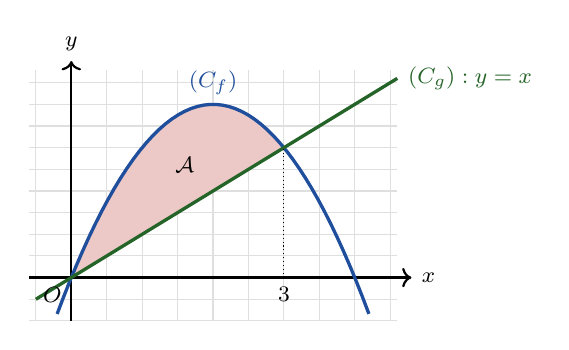
\begin{tikzpicture}[x=0.9cm,y=0.55cm,font=\footnotesize]
\draw[gray!25,step=0.5] (-0.6,-1) grid (4.6,4.8);
\fill[cThm!25] plot[domain=0:3,samples=50] (\x,{-\x*\x+4*\x}) -- plot[domain=3:0,samples=10] (\x,\x) -- cycle;
\draw[->,thick] (-0.6,0)--(4.8,0) node[right]{$x$}; \draw[->,thick] (0,-1)--(0,5) node[above]{$y$};
\draw[cDef,very thick,domain=-0.2:4.2,samples=50] plot (\x,{-\x*\x+4*\x}); \node[cDef] at (2,4.5){$(C_f)$};
\draw[cRem!80!black,very thick] (-0.5,-0.5)--(4.6,4.6) node[right]{$(C_g):y=x$};
\draw[densely dotted] (3,0)--(3,3); \node[below] at (3,0){$3$}; \node[below left] at (0,0){$O$};
\node at (1.6,2.6){$\mathcal A$};
\end{tikzpicture}
\end{FIG}
\[\mathcal A=\int_0^3\big[f(x)-g(x)\big]dx=\int_0^3(-x^2+3x)\,dx=\left[-\frac{x^3}{3}+\frac32x^2\right]_0^3=-9+\frac{27}{2}=\bx{\frac92\ \text{u.a}}\]
\end{mithal}

%================================================================
\origNeedspace{26\baselineskip}\section{تمارين محلولة}
\begin{tmr}
الكلفة الهامشية لإنتاج $q$ مئة وحدة ($0\le q\le10$) هي $C_m(q)=3q^2-24q+60$ (بآلاف الدنانير)، والكلفة الثابتة $50$ ألف دينار.
\QQ{1} بيّن أن $C_m(q)=3(q-4)^2+12$ ، واستنتج اتجاه تغير الكلفة الإجمالية $C$.
\QQ{2} عيّن الكلفة الإجمالية $C(q)$.
\QQ{3} احسب $\displaystyle\int_2^6C_m(q)\,dq$ وفسّر النتيجة اقتصاديًا.
\QQ{4} احسب القيمة المتوسطة للكلفة الهامشية على المجال $[2;6]$.
\end{tmr}
\begin{hal}
\QQ{1} $3(q-4)^2+12=3(q^2-8q+16)+12=3q^2-24q+48+12=3q^2-24q+60=C_m(q)$ \ok.

$C'(q)=C_m(q)=3(q-4)^2+12\ge12>0$ ، إذن \bxt{$C$ متزايدة تمامًا على $[0;10]$}.

\QQ{2} $C$ دالة أصلية لـ $C_m$: \ $C(q)=q^3-12q^2+60q+c$ ، و$C(0)=c=50$ (الكلفة الثابتة):
\[\bx{C(q)=q^3-12q^2+60q+50}\]

\QQ{3} $\displaystyle\int_2^6C_m(q)\,dq=\Big[q^3-12q^2+60q\Big]_2^6=(216-432+360)-(8-48+120)=144-80=\bx{64}$.

\textbf{التفسير:} $\displaystyle\int_2^6C_m(q)\,dq=C(6)-C(2)=194-130=64$: \bxt{زيادة الكلفة الإجمالية $64$ ألف دينار لما ينتقل الإنتاج من $200$ إلى $600$ وحدة}. وهي أيضًا مساحة الحيز الملوّن ($C_m>0$):
\begin{FIG}
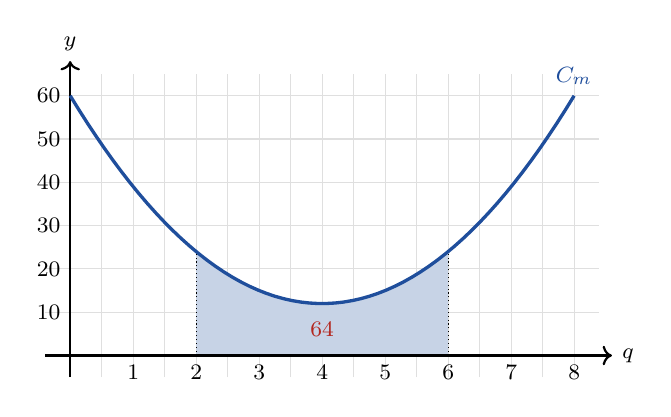
\begin{tikzpicture}[x=0.8cm,y=0.055cm,font=\footnotesize]
\draw[gray!25,xstep=0.5,ystep=10] (-0.4,-5) grid (8.4,65);
\fill[cDef!25] (2,0) -- plot[domain=2:6,samples=50] (\x,{3*\x*\x-24*\x+60}) -- (6,0) -- cycle;
\draw[->,thick] (-0.4,0)--(8.6,0) node[right]{$q$}; \draw[->,thick] (0,-5)--(0,68) node[above]{$y$};
\foreach \t in {1,...,8} \node[below] at (\t,0){$\t$};
\foreach \t in {10,20,...,60} \node[left] at (0,\t){$\t$};
\draw[cDef,very thick,domain=0:8,samples=60] plot (\x,{3*\x*\x-24*\x+60}) node[above]{$C_m$};
\draw[densely dotted] (2,0)--(2,24) (6,0)--(6,24);
\node[cThm] at (4,6){$64$};
\end{tikzpicture}
\end{FIG}
\QQ{4} $\mu=\dfrac{1}{6-2}\displaystyle\int_2^6C_m(q)\,dq=\dfrac{64}{4}=\bx{16}$ ألف دينار: متوسط الكلفة الهامشية بين $200$ و$600$ وحدة.
\end{hal}

\begin{tmr}
$f(x)=x^2-4x+3$ و$g(x)=x-1$ ، $(C_f)$ و$(C_g)$ تمثيلاهما في معلم متعامد $(O;\vec i,\vec j)$ حيث $\|\vec i\|=2\,\text{cm}$ و$\|\vec j\|=1\,\text{cm}$.
\QQ{1} احسب مساحة الحيز المحدد بـ $(C_f)$ ومحور الفواصل والمستقيمين $x=0$ و$x=3$.
\QQ{2} عيّن فاصلتي نقطتي تقاطع $(C_f)$ و$(C_g)$ ، ثم ادرس الوضع النسبي لهما.
\QQ{3} احسب بـ $\text{cm}^2$ مساحة الحيز المحصور بين $(C_f)$ و$(C_g)$.
\end{tmr}
\begin{hal}
\QQ{1} $f(x)=(x-1)(x-3)$:
\begin{FIG}
\begin{tikzpicture}[font=\normalsize]
\fill[gray!12] (0,0) rectangle (2.6,-0.9);
\fill[green!18] (2.6,0) rectangle (15.5,-0.9);
\fill[orange!45] (0,-0.9) rectangle (2.6,-4.6);
\fill[cyan!22] (2.6,-0.9) rectangle (15.5,-4.6);
\draw[thick] (0,0) rectangle (15.5,-4.6); \draw (0,-0.9)--(15.5,-0.9) (0,-1.8)--(15.5,-1.8) (2.6,0)--(2.6,-4.6);
\node at (1.3,-0.45){$x$};
\node at (1.3,-1.35){$f(x)$};
\node[align=center,font=\bfseries] at (1.3,-3.2){\ar{الوضع}\\ \ar{النسبي}};
\node at (3.3,-0.45){$0$};
\node at (7.49355,-0.45){$1$};
\node at (13.3,-0.45){$3$};
\node at (4.64677,-1.35){$+$};
\node[align=center,font=\small] at (4.64677,-3.2){$(C_f)$\\ \ar{فوق}\\ $(xx')$};
\node at (10.3968,-1.35){$-$};
\node[align=center,font=\small] at (10.3968,-3.2){$(C_f)$\\ \ar{تحت}\\ $(xx')$};
\node at (7.49355,-1.35){$0$};
\draw[densely dotted] (7.49355,-0.9)--(7.49355,-1.13) (7.49355,-1.57)--(7.49355,-1.8);
\draw (5.99355,-4.6) .. controls (6.06855,-3.06) and (7.04355,-2.136) .. (7.49355,-1.8) .. controls (7.94355,-2.136) and (8.91855,-3.06) .. (8.99355,-4.6);
\node[align=center,font=\footnotesize,inner sep=0pt] at (7.49355,-3.65){\ar{$(C_f)$ يقطع}\\ $(xx')$\\ \ar{في النقطة}\\ $A(1;0)$};
\node at (13.3,-1.35){$0$};
\draw[densely dotted] (13.3,-0.9)--(13.3,-1.13) (13.3,-1.57)--(13.3,-1.8);
\draw (11.8,-4.6) .. controls (11.875,-3.06) and (12.85,-2.136) .. (13.3,-1.8) .. controls (13.75,-2.136) and (14.725,-3.06) .. (14.8,-4.6);
\node[align=center,font=\footnotesize,inner sep=0pt] at (13.3,-3.65){\ar{$(C_f)$ يقطع}\\ $(xx')$\\ \ar{في النقطة}\\ $B(3;0)$};
\end{tikzpicture}
\end{FIG}
\[\mathcal A_1=\int_0^1f(x)\,dx=\left[\frac{x^3}{3}-2x^2+3x\right]_0^1=\frac13-2+3=\frac43\]
\[\mathcal A_2=-\int_1^3f(x)\,dx=-\Big[(9-18+9)-\frac43\Big]=\frac43\qquad\Longrightarrow\qquad\bx{\mathcal A=\frac83\ \text{u.a}=\frac{16}{3}\,\text{cm}^2}\]
\QQ{2} $f(x)=g(x)$ معناه $x^2-5x+4=0$ أي $(x-1)(x-4)=0$: \ $x=1$ أو $x=4$.

$f(x)-g(x)=(x-1)(x-4)$:
\begin{FIG}
\begin{tikzpicture}[font=\normalsize]
\fill[gray!12] (0,0) rectangle (2.6,-0.9);
\fill[green!18] (2.6,0) rectangle (15.5,-0.9);
\fill[orange!45] (0,-0.9) rectangle (2.6,-4.6);
\fill[cyan!22] (2.6,-0.9) rectangle (15.5,-4.6);
\draw[thick] (0,0) rectangle (15.5,-4.6); \draw (0,-0.9)--(15.5,-0.9) (0,-1.8)--(15.5,-1.8) (2.6,0)--(2.6,-4.6);
\node at (1.3,-0.45){$x$};
\node at (1.3,-1.35){$f(x)-g(x)$};
\node[align=center,font=\bfseries] at (1.3,-3.2){\ar{الوضع}\\ \ar{النسبي}};
\node at (3.3,-0.45){$-\infty$};
\node at (6.69773,-0.45){$1$};
\node at (11.4023,-0.45){$4$};
\node at (14.8,-0.45){$+\infty$};
\node at (4.37386,-1.35){$+$};
\node[align=center,font=\footnotesize] at (4.37386,-3.2){$(C_f)$\\ \ar{فوق}\\ $(C_g)$};
\node at (9.05,-1.35){$-$};
\node[align=center,font=\footnotesize] at (9.05,-3.2){$(C_f)$\\ \ar{تحت}\\ $(C_g)$};
\node at (13.7261,-1.35){$+$};
\node[align=center,font=\footnotesize] at (13.7261,-3.2){$(C_f)$\\ \ar{فوق}\\ $(C_g)$};
\node at (6.69773,-1.35){$0$};
\draw[densely dotted] (6.69773,-0.9)--(6.69773,-1.13) (6.69773,-1.57)--(6.69773,-1.8);
\draw (5.44773,-4.6) .. controls (5.51023,-3.06) and (6.32273,-2.136) .. (6.69773,-1.8) .. controls (7.07273,-2.136) and (7.88523,-3.06) .. (7.94773,-4.6);
\node[align=center,font=\scriptsize,inner sep=0pt] at (6.69773,-3.65){\ar{$(C_f)$ يقطع}\\ $(C_g)$\\ \ar{في النقطة}\\ $A(1;0)$};
\node at (11.4023,-1.35){$0$};
\draw[densely dotted] (11.4023,-0.9)--(11.4023,-1.13) (11.4023,-1.57)--(11.4023,-1.8);
\draw (10.1523,-4.6) .. controls (10.2148,-3.06) and (11.0273,-2.136) .. (11.4023,-1.8) .. controls (11.7773,-2.136) and (12.5898,-3.06) .. (12.6523,-4.6);
\node[align=center,font=\scriptsize,inner sep=0pt] at (11.4023,-3.65){\ar{$(C_f)$ يقطع}\\ $(C_g)$\\ \ar{في النقطة}\\ $B(4;3)$};
\end{tikzpicture}
\end{FIG}
\QQ{3} على $[1;4]$: $(C_g)$ فوق $(C_f)$:
\begin{FIG}
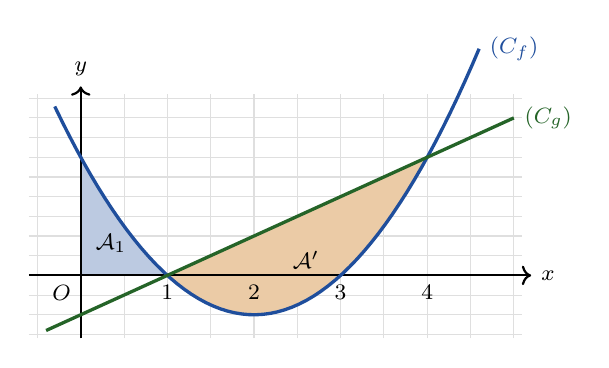
\begin{tikzpicture}[x=1.1cm,y=0.5cm,font=\footnotesize]
\draw[gray!25,step=0.5] (-0.6,-1.6) grid (5.1,4.6);
\fill[cDef!30] (0,0) -- plot[domain=0:1,samples=40] (\x,{\x*\x-4*\x+3}) -- cycle;
\fill[cEx!35] plot[domain=1:4,samples=10] (\x,{\x-1}) -- plot[domain=4:1,samples=50] (\x,{\x*\x-4*\x+3}) -- cycle;
\draw[->,thick] (-0.6,0)--(5.2,0) node[right]{$x$}; \draw[->,thick] (0,-1.6)--(0,4.8) node[above]{$y$};
\draw[cDef,very thick,domain=-0.3:4.6,samples=60] plot (\x,{\x*\x-4*\x+3}) node[right]{$(C_f)$};
\draw[cRem!80!black,very thick] (-0.4,-1.4)--(5,4) node[right]{$(C_g)$};
\foreach \t in {1,...,4} \node[below] at (\t,0){$\t$}; \node[below left] at (0,0){$O$};
\node at (0.35,0.8){$\mathcal A_1$}; \node at (2.6,0.4){$\mathcal A'$};
\end{tikzpicture}
\end{FIG}
\[\mathcal A'=\int_1^4\big[g(x)-f(x)\big]dx=\int_1^4(-x^2+5x-4)\,dx=\left[-\frac{x^3}{3}+\frac52x^2-4x\right]_1^4\]
\[=\left(-\frac{64}{3}+40-16\right)-\left(-\frac13+\frac52-4\right)=\frac83+\frac{11}{6}=\frac92\ \text{u.a}\]
وبما أن $1\ \text{u.a}=2\times1=2\,\text{cm}^2$: \ \bx{\mathcal A'=\frac92\times2=9\,\text{cm}^2}.
\end{hal}

%================================================================
\section{أخطاء شائعة}
\begin{BOX}{cThm}{تجنّب هذه الأخطاء}
\begin{enumerate}[label=\textbf{\arabic*.}]
\item نسيان الثابت $c$ قبل استعمال شرط مثل $F(x_0)=y_0$ أو الكلفة الثابتة $C(0)$.
\item دالة أصلية لـ $\dfrac1{x^2}$ هي $-\dfrac1x$ (لا $\dfrac1x$)، ولـ $\dfrac1{\sqrt x}$ هي $2\sqrt x$ (لا $\dfrac12\sqrt x$).
\item دالة أصلية لجداء ليست جداء الدوال الأصلية: نبحث عن الشكل $u'u^n$ أو نَنشر.
\item نسيان معامل $u'$: دالة أصلية لـ $(3x-1)^2$ هي $\dfrac{(3x-1)^3}{9}$ (لأن $u'=3$) لا $\dfrac{(3x-1)^3}{3}$.
\item حساب $F(a)-F(b)$ بدل $F(b)-F(a)$.
\item أخذ التكامل مساحةً دون دراسة الإشارة: إذا كانت $f\le0$ نأخذ $-\int$، وإذا تغيرت الإشارة نقسم المجال.
\item في المساحة بين منحنيين: طرح الأعلى من الأسفل؛ الصحيح «الأعلى ناقص الأسفل» حسب جدول الوضع النسبي.
\item نسيان تحويل $\text{u.a}$ إلى $\text{cm}^2$ حسب وحدتي المحورين.
\item في القيمة المتوسطة: نسيان القسمة على $b-a$.
\end{enumerate}
\end{BOX}

\origNeedspace{22\baselineskip}\section{خلاصة الطرائق}
\begin{BOX}{cMeth}{الطريقة حسب المطلوب}
\begin{center}
\renewcommand{\arraystretch}{1.35}
\begin{tabular}{|p{0.62\textwidth}|p{0.3\textwidth}|}\hline
\rowcolor{cSec!12} \textbf{الطريقة} & \textbf{المطلوب}\\\hline
نحسب $F'(x)$ ونبيّن أن $F'(x)=f(x)$ على $I$. & التحقق أن $F$ دالة أصلية لـ $f$\\\hline
الجدول + الخطية حدًّا حدًّا؛ أو نتعرف على $u'u^n$ ، $\frac{u'}{u^n}$ ، $\frac{u'}{\sqrt u}$. & تعيين دالة أصلية\\\hline
$F=G+c$ ثم نعوض الشرط $F(x_0)=y_0$ لإيجاد $c$. & دالة أصلية تحقق شرطًا\\\hline
$C$ دالة أصلية لـ $C_m$ ، والكلفة الثابتة $C(0)$ تعيّن الثابت. & الكلفة الإجمالية من الكلفة الهامشية\\\hline
$\int_a^bf(x)\,dx=F(b)-F(a)$. & حساب تكامل\\\hline
$\mu=\frac{1}{b-a}\int_a^bf(x)\,dx$. & القيمة المتوسطة\\\hline
جدول الوضع النسبي (إشارة $f$)، رسم وتلوين، ثم $\int f$ أو $-\int f$ وعلاقة شال. & مساحة بين منحنٍ ومحور الفواصل\\\hline
نقط التقاطع، إشارة $f-g$، ثم تكامل (الأعلى ناقص الأسفل). & مساحة بين منحنيين\\\hline
$1\ \text{u.a}=\|\vec i\|\times\|\vec j\|$. & التحويل إلى $\text{cm}^2$\\\hline
\end{tabular}
\end{center}
\end{BOX}
\end{document}
